%++++++++++++++++++++++++++++++++++++++++
\documentclass[article, 12pt]{article}
\usepackage{float}
\usepackage{setspace}
\usepackage{tabu} % extra features for tabular environment
\usepackage{amsmath}  % improve math presentation
\usepackage{graphicx} % takes care of graphic including machinery
\usepackage[margin=1in]{geometry} % decreases margins
\usepackage{cite} % takes care of citations
\usepackage[final]{hyperref} % adds hyper links inside the generated pdf file
\usepackage{tikz}
\usepackage{caption} 
\usepackage{fancyhdr}
\usepackage{amssymb} % symbols like /therefore
\usepackage{amsthm} % proofs
\usepackage{enumerate} % lettered lists
\usepackage{mathtools} % macros
\usepackage[ all]{xy} % for diagrams
\usepackage{tkz-graph}
\usetikzlibrary{knots}
\usepackage{xcolor}
\usetikzlibrary{scopes}
% \usepackage{xcolor} \pagecolor[rgb]{0.12549019607,0.1294117647,0.13725490196} \color[rgb]{0.82352941176,0.76862745098,0.62745098039} % dark theme
\theoremstyle{definition}
\newtheorem{example}{Example}[subsubsection]
\newtheorem*{remark}{Remark}
\newtheorem{theorem}{Theorem}[subsubsection]
\newtheorem{definition}{Definition}[subsubsection]
\newtheorem{corollary}{Corollary}[subsubsection]
\hypersetup{
	colorlinks=false,      % false: boxed links; true: colored links
	linkcolor=blue,        % color of internal links
	citecolor=blue,        % color of links to bibliography
	filecolor=magenta,     % color of file links
	urlcolor=blue         
}
\usepackage{physics}
\usepackage{siunitx}
\usepackage{tikz,pgfplots}
\usepackage[outline]{contour} % glow around text
\usetikzlibrary{calc}
\usetikzlibrary{angles,quotes} % for pic
\usetikzlibrary{arrows.meta}
\tikzset{>=latex} % for LaTeX arrow head
\contourlength{1.2pt}

\colorlet{xcol}{blue!70!black}
\colorlet{vcol}{green!60!black}
\colorlet{myred}{red!70!black}
\colorlet{myblue}{blue!70!black}
\colorlet{mygreen}{green!70!black}
\colorlet{mydarkred}{myred!70!black}
\colorlet{mydarkblue}{myblue!60!black}
\colorlet{mydarkgreen}{mygreen!60!black}
\colorlet{acol}{red!50!blue!80!black!80}
\tikzstyle{CM}=[red!40!black,fill=red!80!black!80]
\tikzstyle{xline}=[xcol,thick,smooth]
\tikzstyle{mass}=[line width=0.6,red!30!black,fill=red!40!black!10,rounded corners=1,
                  top color=red!40!black!20,bottom color=red!40!black!10,shading angle=20]
\tikzstyle{faded mass}=[dashed,line width=0.1,red!30!black!40,fill=red!40!black!10,rounded corners=1,
                        top color=red!40!black!10,bottom color=red!40!black!10,shading angle=20]
\tikzstyle{rope}=[brown!70!black,very thick,line cap=round]
\def\rope#1{ \draw[black,line width=1.4] #1; \draw[rope,line width=1.1] #1; }
\tikzstyle{force}=[->,myred,very thick,line cap=round]
\tikzstyle{velocity}=[->,vcol,very thick,line cap=round]
\tikzstyle{Fproj}=[force,myred!40]
\tikzstyle{myarr}=[-{Latex[length=3,width=2]},thin]
\def\tick#1#2{\draw[thick] (#1)++(#2:0.12) --++ (#2-180:0.24)}
\DeclareMathOperator{\sn}{sn}
\DeclareMathOperator{\cn}{cn}
\DeclareMathOperator{\dn}{dn}
\def\N{80} % number of samples in plots


\usepackage{titling}
\renewcommand\maketitlehooka{\null\mbox{}\vfill}
\renewcommand\maketitlehookd{\vfill\null}
\usepackage{siunitx} % units
\usepackage{verbatim} 
\newcommand{\courseNumber}{MATH 1700}
\newcommand{\courseName}{Ideas in Mathematics}
\newcommand{\professor}{Professor Rimmer}
\newcommand{\psetName}{Take-Home Final Exam}
\newcommand{\dueDate}{Due: May 5, 2023}
\newcommand{\name}{Denny Cao}
\pagestyle{fancy}
\fancyhf{}% clears all header and footer fields
\fancyfoot[C]{--~\thepage~--}
\renewcommand*{\headrulewidth}{0.4pt}
\renewcommand*{\footrulewidth}{0pt}
\lhead{\name}
\chead{\courseNumber: \courseName}
\rhead{\professor}

% new theorem for questions and answers

\newtheorem{question}{Question}

\newtheorem{answer}{Answer}

\fancypagestyle{plain}{%
  \fancyhf{}% clears all header and footer fields
  \fancyfoot[C]{--~\thepage~--}%
  \renewcommand*{\headrulewidth}{0pt}%
  \renewcommand*{\footrulewidth}{0pt}%
}

% Shortcuts
\DeclarePairedDelimiter\ceil{\lceil}{\rceil} % ceil function
\DeclarePairedDelimiter\floor{\lfloor}{\rfloor} % floor function

\DeclarePairedDelimiter\paren{(}{)} % parenthesis

\newcommand{\df}{\displaystyle\frac} % displaystyle fraction
\newcommand{\qeq}{\overset{?}{=}} % questionable equality

\newcommand{\Mod}[1]{\;\mathrm{mod}\; #1} % modulo operator

\newcommand{\comp}{\circ} % composition

% Sets
\DeclarePairedDelimiter\set{\{}{\}}
\newcommand{\unite}{\cup}
\newcommand{\inter}{\cap}

\newcommand{\reals}{\mathbb{R}} % real numbers: textbook is Z^+ and 0
\newcommand{\ints}{\mathbb{Z}}
\newcommand{\nats}{\mathbb{N}}
\newcommand{\rats}{\mathbb{Q}}

\newcommand{\degree}{^\circ}

% Counting
\newcommand\perm[2][^n]{\prescript{#1\mkern-2.5mu}{}P_{#2}}
\newcommand\comb[2][^n]{\prescript{#1\mkern-0.5mu}{}C_{#2}}

% Relations
\newcommand{\rel}{\mathcal{R}} % relation

\setlength\parindent{0pt}

% Directed Graphs
\usetikzlibrary{arrows}
\tikzset{vertex/.style = {shape=circle,draw, minimum size=1.5em,
inner sep=0pt, outer sep=0pt}}
\tikzset{edge/.style = {->,> = latex'}}

% Contradiction
\newcommand{\contradiction}{{\hbox{%
    \setbox0=\hbox{$\mkern-3mu\times\mkern-3mu$}%
    \setbox1=\hbox to0pt{\hss$\times$\hss}%
    \copy0\raisebox{0.5\wd0}{\copy1}\raisebox{-0.5\wd0}{\box1}\box0
}}}

% Sign Charts
\newdimen\tcolw \tcolw=2.5em % the column width
\edef\ecatcode{\catcode`&=\the\catcode`&\relax}\catcode`&=4
\def\sgchart#1#2{\vbox{\offinterlineskip\halign{\hfil##\quad&##\hfil\crcr\sgchartA#2,:,%
   \omit\sgchartR&\kern.2pt\sgchartS{.5\tcolw}\relax\sgchartE#1,\relax,%
   \sgchartS{.5\tcolw}\relax\cr
   \noalign{\kern2pt}&\def~{}\kern.5\tcolw\sgchartD#1,\relax,\cr}}}
\def\sgchartA#1:#2,{\cr\ifx,#1,\else $#1$&\sgchartB#2{}\expandafter\sgchartA\fi}
\def\sgchartB#1{\hbox to\tcolw{\hss$#1$\hss}\sgchartC}
\def\sgchartC#1{\ifx,#1,\else
   \strut\vrule\kern-.4pt\hbox to\tcolw{\hss$#1$\hss}\expandafter\sgchartC\fi}
\def\sgchartD#1#2,{\ifx\relax#1\else\hbox to\tcolw{\hss$#1#2$\hss}\expandafter\sgchartD\fi}
\def\sgchartE#1#2,{\ifx\relax#1\else
    \ifx~#1\sgchartS\tcolw\circ \else\sgchartS\tcolw\bullet\fi \expandafter\sgchartE\fi}
\def\sgchartR{\leaders\vrule height2.8pt depth-2.4pt\hfil}
\def\sgchartS#1#2{\hbox to#1{\kern-.2pt\sgchartR \ifx\relax#2\else
   \kern-.7pt$#2$\kern-.7pt\sgchartR\fi\kern-.2pt}}
\ecatcode
%++++++++++++++++++++++++++++++++++++++++
% title stuff

\makeatletter
\renewcommand{\maketitle}{\bgroup\setlength{\parindent}{0pt}
    \begin{flushleft}
        \textbf{\@title} \\ \vskip0.2cm
        \begingroup
            \fontsize{14pt}{12pt}\selectfont
            \courseNumber: \courseName 
            \vskip0.3cm 
            \professor
        \endgroup \vskip0.3cm
        \dueDate \hfill\rlap{}\bf{\name} \\ \vskip0.1cm
        \hrulefill
    \end{flushleft}\egroup 
}
\makeatother

\title{\Large\bf{\psetName}}

\begin{document}
    \maketitle
    \thispagestyle{plain}
    \section{Reflection}
    % Reflection Q1
    \begin{question}
        Has your understanding of mathematics as a discipline changed as a result of taking the course? If so, how? If not, why not?
    \end{question}
    % Reflection A1
    \begin{answer}
        Mathematics to me used to be about memorizing formulas and proofs and then applying them to solve problems. However, after MATH 1700, I now realize that mathematics is more than just that.
        \\[12pt]
        Mathematics is a way of thinking, a tool to solve problems, a language to describe the world around us. I've learned about the underlying concepts and principles that govern mathematics. I've begun to appreciate the elegance and beauty of mathematics. (I also now plan to double major in applied mathematics and computer science!)
        \\[12pt]
        This course has also taught me the importance of critical thinking and problem-solving skills in mathematics. I now attempt to approach problems in a structured and logical manner and creatively when faced with challenging problems. This has helped me to not only excel in this course but also to apply these skills in other areas of my academic and personal life.
    \end{answer}

    % Reflection Q2
    \begin{question}
        What topic(s) from this class did you find most interesting, and why?    
    \end{question}
    % Reflection A2
    \begin{answer}
        I found Knot Theory and the Art Gallery Theorem interesting, as they were the two topics that I was unfamiliar with. 
        \\[12pt] 
        Knot Theory was a completely different way of thinking. Initially, I attempted to understand it by relating it to directed graphs, but it didn't work and I realized I would have to actually use knot diagrams. I also thought that the concept was not that useful until I Googled the applications of Knot Theory, being used to study DNA, the behavior of polymers, the flow of fluids, and the properties of materials. 
        \\[12pt]
        The Art Gallery Theorem was fascinating because it allowed me to quantitatively evaluate something I previously relied on intuition for. In games like Balloon Tower Defense, I would place towers in a way that I thought would cover the most area, but I now know mathematically how many towers I would need to ensure balloons could be popped anywhere on the map.
    \end{answer}
    
    % Reflection Q3
    \begin{question}
        Choose a mathematical topic you are curious about that was not covered in this class, and outline some steps you could take to learn more about it.
    \end{question}
    % Reflection A3
    \begin{answer}
        I'm interested in learning linear algebra. Currently, I'm following along with Gilbert Strang's lectures on MIT OpenCourseWare for 18.06 Linear Algebra. After I finish lectures, I write notes and complete practice problebms. I'm planning on incorporating the Feynman Technique into my learning process by explaining topics to myself in simple terms and using analogies to relate them to concepts I already understand, sort of like what we did in MATH 1700.
    \end{answer}

    % Reflection Q4 
    \begin{question}
        Take one homework problem you worked on this semester that you struggled to understand and/or solve, and explain how that struggle was beneficial.
    \end{question}
    % Reflection A4
    \begin{answer}
        I originally couldn't figure out a solution for Question 13 for p-set 4 about Cardinality: You come across a previously undiscovered ancient language. The language appears to have four letters, which can be used in any order to form words. There is no known limit on the number of letters per word, although each individual word may only have finitely many letters. Explain why the set of all possible words in this language is countable. 
        \\[12pt]
        After some thinking, I decided to apply what I learned in discrete mathematics with number theory. I initially used base 4, but then realized that there were some ambiguities in base 4. For instance, ``abba'' and ``bba'' would have the same base 4 representation, $110_4$. Instead, I used base 5. The base 5 number could then be converted to base 10, which each unique word would have a unique base 10 representation. I was extremely proud when I solved the problem, utilizing past knowledge and being able to formualte a solution from that. It was also so cool to see everything come together to solve the problem.
    \end{answer}

    % Reflection Q5
    \begin{question}
        During this semester, did you change your approach to the class? If so, how? If you were to retake this class, would you approach it differently?
    \end{question}
    % Reflection A5
    \begin{answer}
        I initially worked on the p-sets by myself, but I realized that I was spending a lot of time on problems that I couldn't solve. I would go and review notes and read my discrete mathematics textbook, watch videos, and search on Google for similar questions. I then started working with a group of friends, and we would discuss problems and help each other when we got stuck. This was extremely beneficial, as I was able to learn from my peers and also teach them concepts that they were unfamiliar with. I immediately started to see an improvement, as I no longer would spend long periods of time on a single problem.
        \\[12pt]
        If I were to retake this class, I would start working with a group of friends from the beginning of the semester. We would be able to learn quicker and more efficiently. Learning would also be more fun and enjoyable, as we would be able to discuss problems and concepts with each other.
    \end{answer}

    % Reflection Q6
    \begin{question}
        Are there any skills or behaviors that you learned or modified in this class that might be
        beneficial to you in other courses, or in life more generally? Elaborate.
    \end{question}
    % Reflection A6
    \begin{answer}
        This school year was my first introduction to proof writing in mathematics through my discrete mathematics course at Community College of Philadelphia. My proofs were extremely complicated, filled with mathematical jargon and concepts and, when helping others with the p-sets, I would have to take a lot of time to explain my proofs to them. During exams, I would sometimes have a few points deduced for being extremely verbose!
        \\[12pt]
        Taking this class has taught me to become more clear and more concise with proofs, challenging me to teach mathematical concepts to someone who is unfamiliar with said concepts. 
    \end{answer}

    % Reflection Q7
    \begin{question}
        Ten years from now, you probably will not remember Cantor's diagonal argument nor how to three-color a knot diagram. What lessons from this class, if any, do you hope to retain for years and years to come?   
    \end{question}
    % Reflection A7
    \begin{answer}
        Although, I will probably not remember Cantor's diagonal argument, nor how to three-color a knot diagram, I will remember many lessons I learned from this class. I will remember the importance of critical thinking and problem-solving skills in mathematics. I will remember the importance of collaboration and teamwork in learning. I will remember the importance of clear and concise communication in mathematics. I will remember the importance of creativity and imagination in mathematics. I will remember the importance of curiosity and passion in mathematics. I will remember the importance of mathematics in the world around us.
        \\[12pt]
        Aside from the lessons I learned, there are a few topics that I \textit{will} probably remember. I will remember the Pigeonhole Principle because of the sort of ``common sense'' nature to it (as well as because of the name!). I will probably remember a lot of the graph theory we learned, as graph theory will be fundemental to me as I go on to study computer science at Harvard.
        \\[12pt]
        This class has been a wonderful experience, and I'm extremely grateful to have been a part of it. Mathematics has become even more enjoyable as a subject, and I am even more interested in learning more by working together with others. Thank you for a great semester!
    \end{answer}

    % Reflection Q8
    \begin{question}
        Describe your personal relationship with mathematics as a discipline and/or within mathematics as a community. Do you feel that this relationship has changed during this semester? If so, how? If not, why not?
    \end{question}
    % Reflection A8
    \begin{answer}
        I have personally loved mathematics all my life simply for the fact that there is always more to learn, and that there is a concrete answer but still with multiple approaches to reach that answer. This year, I've taken MATH 163 and 263 at Community College of Philadelphia, and I've learned that mathematics is not just about numbers and equations, but also about logic and reasoning, learning topics from logical expressions, to proofs, to set theory, to number theory, to counting and probability, to graph theory. I've also taken MATH 1410 at Penn and explored deeper into calculus. Learning multivariable calculus has helped me in my physics classes, understanding vector fields, dot products, cross products, as well as Maxwell's equations! Physics has been the real world application of mathematics for me, with derivatives and integrals appearing in kinematics as well as nearly every equation we use. Mathematics has slowly become less of solving equations and more of applying to different topics and concepts, and I've loved every second of it.
        \\[12pt]
        This semester, my love for mathematics has crystalized even more. Math has now become a team sport rather than an individual sport. Its been extremely fun and rewarding to learn together, explain concepts to each other, and solve problems together. 
    \end{answer}

    \section{Graph Theory}
    \setcounter{question}{0}
    \setcounter{answer}{0}
    % Graph Theory Q1
    \begin{question} \
        \begin{enumerate}[(a)]
            \item Does the graph have an Euler path? If not, why not? If so, find one.
            \item Does the graph have an Euler circuit? If not, why not? If so, find one.
        \end{enumerate}
        \begin{figure}[H]
            \centering
            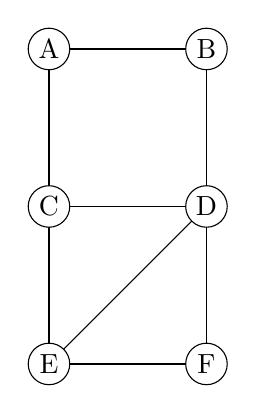
\begin{tikzpicture}
                \node[vertex] (A) at (0,0) {A};
                \node[vertex] (B) at (2,0) {B};
                \node[vertex] (C) at (0,-2) {C};
                \node[vertex] (D) at (2,-2) {D};
                \node[vertex] (E) at (0,-4) {E};
                \node[vertex] (F) at (2,-4) {F};

                \draw (A) to (B);
                \draw (A) to (C);
                \draw (C) to (D);
                \draw (B) to (D);

                \draw (C) to (E);
                \draw (D) to (F);
                \draw (E) to (F);

                \draw (D) to (E);
            \end{tikzpicture}
        \end{figure}
    \end{question}
    % Graph Theory A1
    \begin{answer} \
        \begin{enumerate}[a)]
            \item \begin{proof}
                The degrees of the vertices are as follows:
                \begin{figure}[H]
                    \centering
                    \begin{tabular}{|c|c|}
                        \hline
                        Vertex & Degree \\
                        \hline
                        A & 2 \\
                        B & 2 \\
                        C & 3 \\
                        D & 4 \\
                        E & 3 \\
                        F & 2 \\
                        \hline
                    \end{tabular}
                    \caption{Degrees of the Vertices}
                    \label{fig:dov}
                \end{figure}
                As there are only two vertices with odd degree, by Euler's Path 
                Theorem, there exists at least one Euler path. An Euler path is as follows: $ED, DF, FE, EC, CD, DB, BA$. 
            \end{proof}
            \item \begin{proof}
                From \autoref{fig:dov}, there exists a vertex with odd degree, $C$ and $E$. Therefore, by Euler's Cycle Theorem, there does not exist a Euler circuit.  
            \end{proof}
        \end{enumerate}
    \end{answer}
    \section{Art Gallery Theorem}
    \begin{question} \
        \begin{enumerate}[a)]
            \item Triangulate the gallery below.
            \item Use your triangulation to color the vertices of the gallery as in the proof of the art gallery theorem.
            \item Following the proof of the theorem, use your triangulation to identify where to place the fewest amount of guards who can see the entire gallery. Use stars to indicate where you will place the guards.
        \end{enumerate}
        \begin{figure}[H]
            \centering
            \begin{tikzpicture}[scale=0.25]
                \draw (0, 0) node (A)  {} -- (-2, -5) node (B) {} -- (5, 2) node (C) {} -- (8, -3) node (D) {} -- (5, -5) node (E) {} -- (10, -5) node (F) {} -- (13, -10) node (G) {} -- (10, -15) node (H) {} -- (8, -10) node (I) {} -- (3, -12) node (J) {} -- (-2, -17) node (K) {} -- (-5, -15) node (L) {} -- (-7, -15) node (M) {} -- (-5, -7) node (N) {} -- (-7, -5) node (O) {} -- (0,0);
            \end{tikzpicture}
        \end{figure}
        \begin{answer} \
            \begin{enumerate}[a)] 
                \item \ 
                \begin{figure}[H]
                    \centering
                    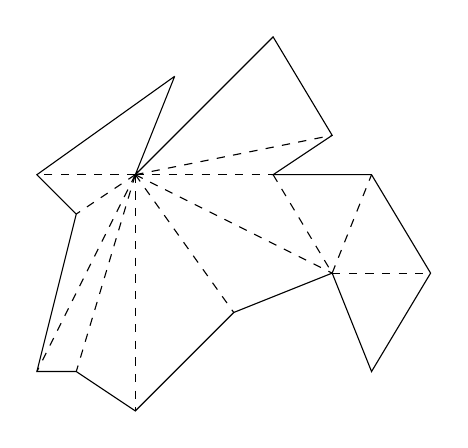
\begin{tikzpicture}[scale=0.25]
                        \draw (0, 0) node (A)  {} -- (-2, -5) node (B) {} -- (5, 2) node (C) {} -- (8, -3) node (D) {} -- (5, -5) node (E) {} -- (10, -5) node (F) {} -- (13, -10) node (G) {} -- (10, -15) node (H) {} -- (8, -10) node (I) {} -- (3, -12) node (J) {} -- (-2, -17) node (K) {} -- (-5, -15) node (L) {} -- (-7, -15) node (M) {} -- (-5, -7) node (N) {} -- (-7, -5) node (O) {} -- (0,0);
                            
                        % B to O
                        \draw[dashed] (-2,-5) -- (-7,-5);
                        % B to N
                        \draw[dashed] (-2,-5) -- (-5,-7);
                        % B to M
                        \draw[dashed] (-2,-5) -- (-7,-15);
                        % B to L
                        \draw[dashed] (-2,-5) -- (-5,-15);
                        % B to K
                        \draw[dashed] (-2,-5) -- (-2,-17);
                        % B to J
                        \draw[dashed] (-2,-5) -- (3,-12);
                        % B to I
                        \draw[dashed] (-2,-5) -- (8,-10);
                        % B to D
                        \draw[dashed] (-2,-5) -- (8,-3);
                        % B to E
                        \draw[dashed] (-2,-5) -- (5,-5);
                        % E to I
                        \draw[dashed] (5,-5) -- (8,-10);
                        % I to F
                        \draw[dashed] (8,-10) -- (10,-5);
                        % I to G
                        \draw[dashed] (8,-10) -- (13,-10);
                    \end{tikzpicture}
                \end{figure}
                \item \
                \begin{figure}[H]
                    \centering
                    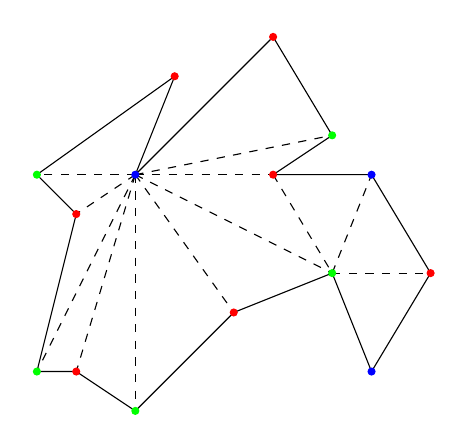
\begin{tikzpicture}[scale=0.25]
                        \draw (0, 0) node (A)  {} -- (-2, -5) node (B) {} -- (5, 2) node (C) {} -- (8, -3) node (D) {} -- (5, -5) node (E) {} -- (10, -5) node (F) {} -- (13, -10) node (G) {} -- (10, -15) node (H) {} -- (8, -10) node (I) {} -- (3, -12) node (J) {} -- (-2, -17) node (K) {} -- (-5, -15) node (L) {} -- (-7, -15) node (M) {} -- (-5, -7) node (N) {} -- (-7, -5) node (O) {} -- (0,0);                            
                        % B to O
                        \draw[dashed] (-2,-5) -- (-7,-5);
                        % B to N
                        \draw[dashed] (-2,-5) -- (-5,-7);
                        % B to M
                        \draw[dashed] (-2,-5) -- (-7,-15);
                        % B to L
                        \draw[dashed] (-2,-5) -- (-5,-15);
                        % B to K
                        \draw[dashed] (-2,-5) -- (-2,-17);
                        % B to J
                        \draw[dashed] (-2,-5) -- (3,-12);
                        % B to I
                        \draw[dashed] (-2,-5) -- (8,-10);
                        % B to D
                        \draw[dashed] (-2,-5) -- (8,-3);
                        % B to E
                        \draw[dashed] (-2,-5) -- (5,-5);
                        % E to I
                        \draw[dashed] (5,-5) -- (8,-10);
                        % I to F
                        \draw[dashed] (8,-10) -- (10,-5);
                        % I to G
                        \draw[dashed] (8,-10) -- (13,-10);
    
                        % Color the vertices
                        % a = red
                        \filldraw[red] (A) circle (5pt);
                        % b = blue
                        \filldraw[blue] (B) circle (5pt);
                        % o = green
                        \filldraw[green] (O) circle (5pt);
                        % n = red
                        \filldraw[red] (N) circle (5pt);
                        % m = green
                        \filldraw[green] (M) circle (5pt);
                        % l = red
                        \filldraw[red] (L) circle (5pt);
                        % k = green
                        \filldraw[green] (K) circle (5pt);
                        % j = red
                        \filldraw[red] (J) circle (5pt);
                        % i = green
                        \filldraw[green] (I) circle (5pt);
                        % e = red
                        \filldraw[red] (E) circle (5pt);
                        % d = green
                        \filldraw[green] (D) circle (5pt);
                        % c = red
                        \filldraw[red] (C) circle (5pt);
                        % f = blue
                        \filldraw[blue] (F) circle (5pt);
                        % g = red
                        \filldraw[red] (G) circle (5pt);
                        % h = blue
                        \filldraw[blue] (H) circle (5pt);
                    \end{tikzpicture}
                \end{figure}
                \item \
                \begin{figure}[H]
                    \centering
                    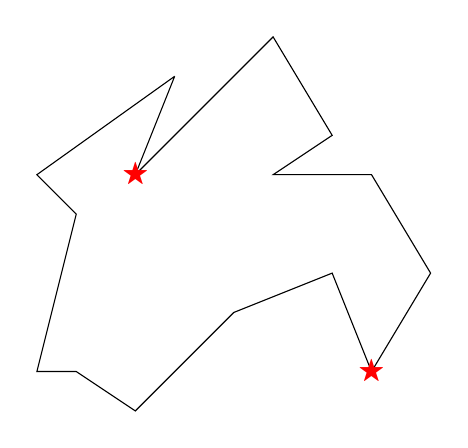
\begin{tikzpicture}[scale=0.25]
                        \draw (0, 0) node (A)  {} -- (-2, -5) node (B) {$\color{red} \bigstar$} -- (5, 2) node (C) {} -- (8, -3) node (D) {} -- (5, -5) node (E) {} -- (10, -5) node (F) {} -- (13, -10) node (G) {} -- (10, -15) node (H) {$\color{red} \bigstar$} -- (8, -10) node (I) {} -- (3, -12) node (J) {} -- (-2, -17) node (K) {} -- (-5, -15) node (L) {} -- (-7, -15) node (M) {} -- (-5, -7) node (N) {} -- (-7, -5) node (O) {} -- (0,0);
                    \end{tikzpicture}
                \end{figure}
            \end{enumerate}
        \end{answer}

    \end{question}
    \section{Pigeonhole Principle}
    % Pigeonhole Principle Q3
    \begin{question}
        I have 7 pairs of socks in my drawer, one of each color of the rainbow. How many socks do I have to draw out in order to guarentee that I have grabbed at least one pair? What if there are likewise colored pairs of gloves in there and I cannot tell the difference between gloves and socks and I want a matching set?
    \end{question}
    % Pigeonhole Principle A3
    \begin{answer}
        \begin{proof} 
            \textbf{If we draw 8 socks, we are guarenteed to have a pair.} This is because it is possible to draw 7 socks of different colors, but if we draw 8 socks, our 8th sock must be the same color as one of the previous 7 socks.
        \end{proof}
        \begin{proof}
            \textbf{If we draw 22 items, we are guarenteed to have a matching set.} This is because it is possible to draw all the gloves before drawing any socks, meaning we could draw 14 items before even drawing a sock. From our previous proof, we know that we are guarenteed to have a pair of socks if we draw 8 socks. As we have already drawn all the gloves, we have a matching set for the pair of socks we drew. Therefore, we are guarenteed to have a matching set if we draw 22 items. 
        \end{proof}
    \end{answer}
\end{document} 
